%!TEX root = thesis.tex

\section{Motivation}

Teaching machines to understand human language documents is one of the most elusive and long-standing challenges in Artificial Intelligence. Before we proceed, we must ask what it means to understand human language? Figure~\ref{fig:mctest-example} demonstrates a children's story from the \sys{MCTest} dataset~\cite{richardson2013mctest}, with simple vocabulary and grammar. To process such a passage of text, the NLP community has put decades of effort into solving different tasks for various aspects of text understanding, including:
\begin{enumerate}[(a)]
    \item
        \tf{part-of-speech tagging}. It requires our machines to understand that, for example, in the first sentence \ti{Alyssa got to the beach after a long trip.}, \ti{Alyssa} is a proper noun, \ti{beach} and \ti{trip} are common nouns, \ti{got} is a verb in its past tense, \ti{long} is an adjective, \ti{after} is a preposition.
    \item
        \tf{named entity recognition}. Our machines also should understand that \ti{Alyssa}, \ti{Ellen}, \ti{Kristen} are the names of people in the story while \ti{Charlotte}, \ti{Atlanta} and \ti{Miami} are the names of locations.
    \item
        \tf{syntactic parsing}. To understand the meaning of each single sentence, our machines also need to understand the relationship between words, or the syntactical (grammatical) structure. Taking the first sentence \ti{Alyssa got to the beach after a long trip.} as an example again, the machines should understand that \ti{Alyssa} is the subject, and \ti{beach} is the object of the verb \ti{got}, while \ti{after a long trip} as a whole is a prepositional phrase which describes a temporal relationship with the verb.
    \item
        \tf{coreference resolution}. Furthermore, our machines even need to understand the interplay between sentences. For example, the mention \ti{She} in the sentence \ti{She's now in Miami} refers to \ti{Alyssa} mentioned in the first sentence, while the mention \ti{The girls} refers to \ti{Alyssa, Ellen, Kristen and Rachel} in the previous sentences.
\end{enumerate}

\begin{figure}[!t]
\center
\begin{tabular}{l p{13cm}}
\toprule
    &{\tf{Alyssa}} got to the beach after a long trip. She's from Charlotte. She traveled from Atlanta. She's now in Miami. She went to Miami to visit some friends. But she wanted some time to herself at the beach, so she went there first. After going swimming and laying out, she went to her friend \tf{Ellen}'s house. \tf{Ellen} greeted {\tf{Alyssa}} and they both had some lemonade to drink. {\tf{Alyssa}} called her friends \tf{Kristen} and \tf{Rachel} to meet at \tf{Ellen}'s house. The girls traded stories and caught up on their lives. It was a happy time for everyone. The girls went to a restaurant for dinner. The restaurant had a special on catfish. \tf{Alyssa} enjoyed the restaurant's special. \tf{Ellen} ordered a salad. \tf{Kristen} had soup. \tf{Rachel} had a steak. After eating, the ladies went back to \tf{Ellen}'s house to have fun. They had lots of fun. They stayed the night because they were tired. {\tf{Alyssa}} was happy to spend time with her friends again. \\
\midrule
  (a) & \tf{Question:} What city is Alyssa in? \\
  &\tf{Answer}: Miami \\
\vspace{0.25em}
  (b) &\tf{Question}: What did Alyssa eat at the restaurant? \\
  & \tf{Answer}: catfish \\
\vspace{0.25em}
  (c) &\tf{Question}: How many friends does Alyssa have in this story? \\
  & \tf{Answer}: 3 \\
\bottomrule
\end{tabular}
\longcaption{A sample story and comprehension questions from \sys{MCTest}}{\label{fig:mctest-example} A sample story and comprehension questions from the \sys{MCTest} dataset  \\ \cite{richardson2013mctest}.}
\end{figure}

Is there a comprehensive evaluation that can test all these aspects and probe even deeper levels of understanding? We argue that the task of \tf{reading comprehension} --- answering comprehension questions over a passage of text --- is a proper and important way to approach that. Just as we use reading comprehension tests to measure how well a human has understood a piece of text, we believe that it can play the same role for evaluating how well computer systems understand human language.

Let's take a closer look at some comprehension questions posed on the same passage (Figure~\ref{fig:mctest-example}):
\begin{enumerate}[(a)]
    \item
        To answer the first question \ti{What city is Alyssa in?}, our machines need to pick out the sentence \ti{She's now in Miami.}, and resolve the \ti{coreference resolution} problem that \ti{She} refers to \ti{Alyssa}, and then finally give the correct answer \ti{Miami}.
    \item
        For the second question \ti{What did Alyssa eat at the restaurant?}, they need to first locate the two sentences \ti{The restaurant had a special on catfish.} and \ti{Alyssa enjoyed the restaurant's special.} and understand the \ti{special} that \ti{Alyssa enjoyed} in the second sentence refers back to the first sentence. Based on the fact that \ti{catfish} modifies \ti{special}, the answer is hence \ti{catfish}.
    \item
        The last question is especially challenging. To arrive at the correct answer, the machines have to keep track of all the names of people mentioned in the text and their relationships, perform some arithmetic reasoning (counting), and finally give the answer \ti{3}.
\end{enumerate}

As we can see, our computer systems have to understand many different aspects of text to answer these questions correctly. Since questions can be designed to query the aspects that we care about, \ti{reading comprehension could be the most suitable task for evaluating language understanding}. This is a central theme of this thesis.

In this thesis, we study the problem of reading comprehension: how can we build computer systems to read a passage and answer these comprehension questions? In particular, we focus on \tf{neural reading comprehension}, a class of reading comprehension models built using deep neural networks, which have been proven much more effective than non-neural, feature-based models.

The field of reading comprehension has a long history --- as early as the 1970s, researchers already recognized that it is an important way to test the language understanding capabilities of computer programs~\cite{lehnert1977process}. However, the field has been neglected for decades and only recently, it has received a great deal of attention and rapid progress has been made (see Figure~\ref{fig:squad-progress} as an example), including our efforts that we will detail in this thesis. The recent success of reading comprehension can be attributed to two reasons: 1) the creation of large-scale supervised datasets in the form of (passage, question, answer) triples; 2) the development of neural reading comprehension models.

In this thesis, we will cover the essence of modern neural reading comprehension: the formulation of the problem, the building blocks and key ingredients of these systems, and understanding of where current neural reading comprehension systems can excel and where they still lag behind.

\begin{figure}[!t]
    \center
    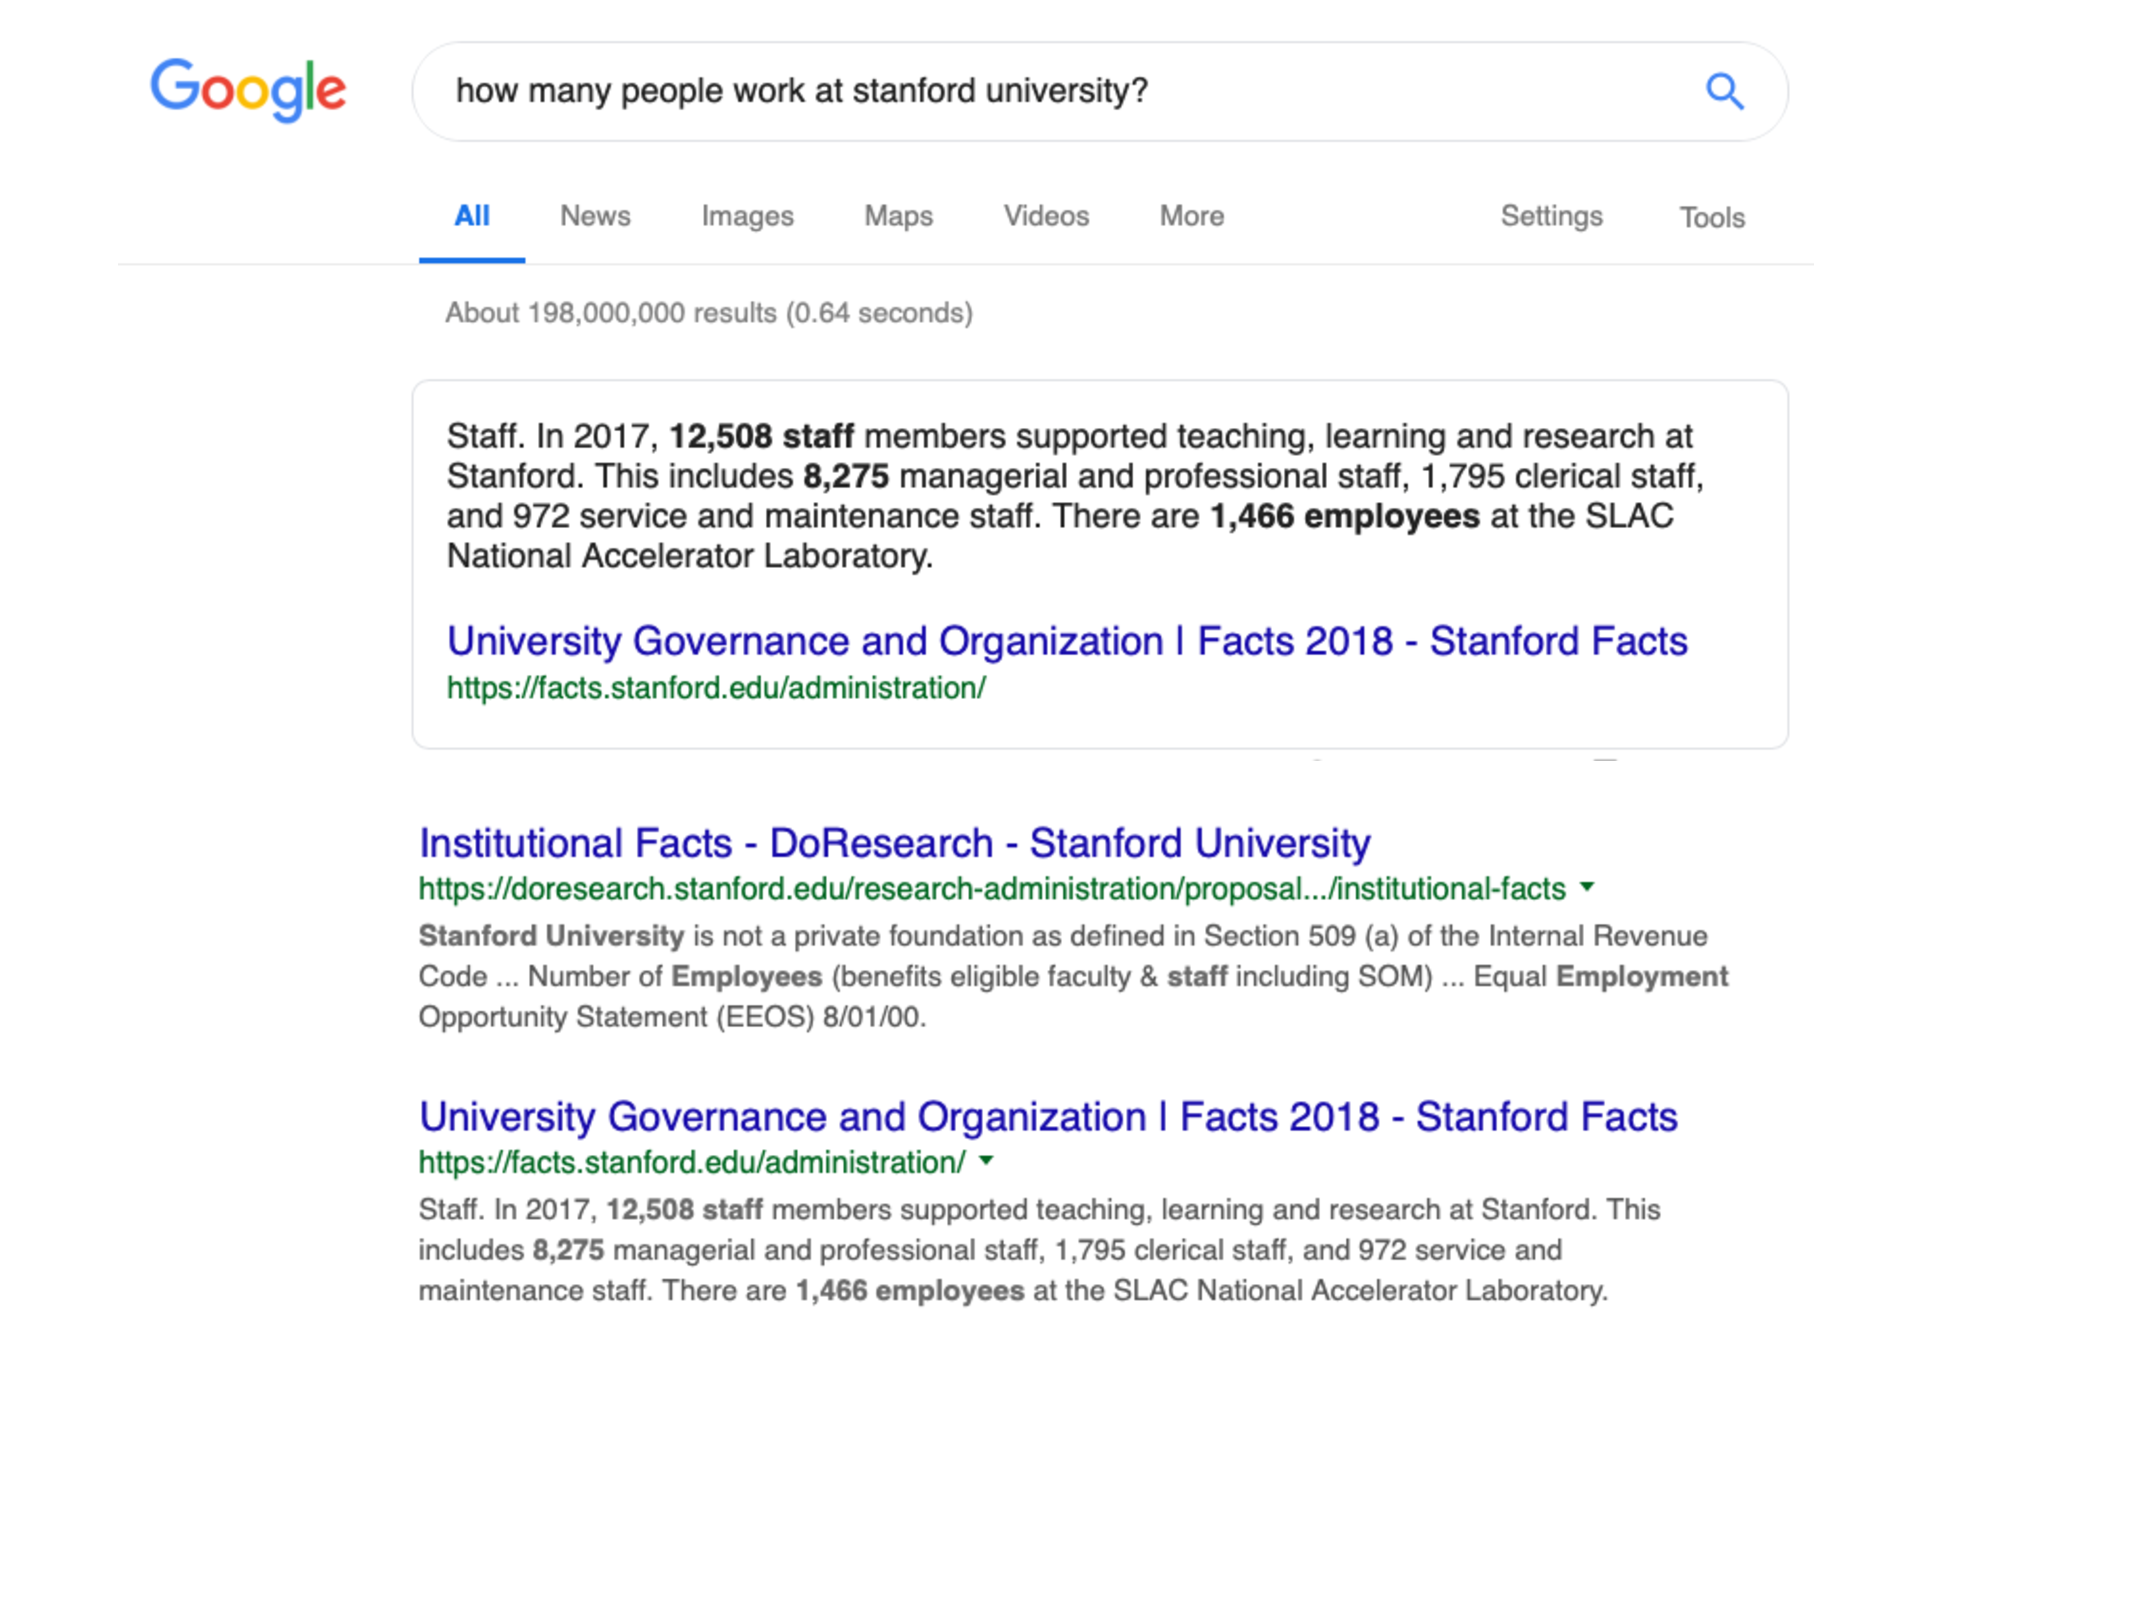
\includegraphics[scale=0.5]{img/google_search.pdf}
    \longcaption{A search result on \sys{Google}}{\label{fig:google-search}A search result on \sys{Google}. It not only returns a list of search documents but gives more precise answers within the documents.}
\end{figure}

The second central theme of the thesis is that we deeply believe that, if we can build high-performing reading comprehension systems, \ti{they would be a crucial technology for applications such as question answering and dialogue systems}. Indeed, these language technologies are already very relevant to our daily lives. For example, today if we enter a search query into \sys{Google} ``How many people work at Stanford University?'' (Figure~\ref{fig:google-search}), \sys{Google} not only returns a list of search documents, but also attempts to read these Web documents and finally highlight the most plausible answers and display them at the top of the search results. We believe this is exactly where reading comprehension can help and thus can facilitate more intelligent search engines. Additionally, with the development of digital personal assistants such as Amazon's \sys{Alexa}, Apple's \sys{Siri}, \sys{Google Assistant} or Microsoft's \sys{Cortana}, more and more users engage with these devices by having conversations and asking informational questions.\footnote{A recent study \href{https://www.stonetemple.com/digital-personal-assistants-study/}{https://www.stonetemple.com/digital-personal-assistants-study/} reported that asking general questions is indeed the number one use for such digital personal assistants.} We believe that building machines which are able to read and comprehend text will also greatly improve the capabilities of these personal assistants.

\begin{figure}[!h]
\small
\center
\begin{tabular}{p{0.85\columnwidth}}
\midrule
Fort Lauderdale, Florida (CNN) -- Just taking a sip of water or walking to the bathroom is excruciatingly painful for 15-year-old Michael Brewer, who was burned over 65 percent of his body after being set on fire, allegedly by a group of teenagers. \\
``It hurts my heart to see him in pain, but it enlightens at the same time to know my son is strong enough to make it through on a daily basis,'' his mother, Valerie Brewer, told CNN on Wednesday. \\
Brewer and her husband, Michael Brewer, Sr., spoke to CNN's Tony Harris, a day after a 13-year-old boy who witnessed last month's attack publicly read a written statement: \\
``I want to express my deepest sympathy to Mikey and his family,'' Jeremy Jarvis said.``I will pray for Mikey to grow stronger every day and for Mikey's speedy recovery.'' \\
Jarvis' older brother has been charged in the October 12 attack in Deerfield Beach, Florida. When asked about the teen's statement, Valerie Brewer -- who knows the Jarvis family -- said she ``can't focus on that.'' \\
``I would really like to stay away from that because that brings negative energy to me and I don't need that right now,'' she said. \\
Her son remains in guarded condition at the University of Miami's Jackson Memorial Hospital Burn Center. He suffered second- and third-degree burns over about two-thirds of his body, according to the hospital's associate director, Dr. Carl Schulman. \\
The teen faces a lifelong recovery from his injuries, Schulman told CNN's Harris.  \\
\vspace{0em}
$Q_1$: What is the subject of the story? \\
$A_1$: Michael Brewer \\
\vspace{0em}
$Q_2$: What happened to him?\\
$A_2$: He was burned \\
\vspace{0em}
$Q_3$: How badly?\\
$A_3$: Over 65\% of his body \\
\vspace{0em}
$Q_4$: Do we know who caused the burns?\\
$A_4$: Yes \\
\bottomrule
\end{tabular}
\longcaption{A conversation from \sys{CoQA} based on an CNN article}{\label{fig:coqa-cnn-example} A conversation from \sys{CoQA} based on an CNN article.}
\end{figure}

Therefore, in this thesis, we are also interested in how we can build practical applications from the recent success of neural reading comprehension. We explore two research directions which employ neural reading comprehension as a key component:
\begin{description}
    \item \tf{Open-domain question answering} combines the challenges from both information retrieval and reading comprehension and aims to answer general questions from either the Web or a large encyclopedia (e.g., Wikipedia).
    \item \tf{Conversational question answering} combines the challenges from dialogue and reading comprehension, and tackles the problem of multi-turn question answering over a passage of text, like how users would engage with conversational agents. Figure~\ref{fig:coqa-cnn-example} demonstrates an example from our \sys{CoQA} dataset~\cite{reddy2019coqa}. In this example, a person can ask a series of interconnected questions based on the content of a \sys{CNN} article.
\end{description}



\section{Thesis Outline}

Following the two central themes that we just discussed, this thesis consists of two parts --- \sys{Part I Neural Reading Comprehension: Foundations} and \sys{Part II Neural Reading Comprehension: Applications}.

\sys{Part I} focuses on the task of reading comprehension, with an emphasis on close reading of a short paragraph so that computer systems are able to answer comprehension questions.
\begin{description}
    \item In Chapter~\ref{chapter:rc-overview}, we first give an overview of the history and recent development of the field of reading comprehension. Next we formally define the problem formulation and its main categories. We then briefly discuss the differences of reading comprehension and general question answering.  Finally, we argue that the recent success of neural reading comprehension is driven by both large-scale datasets and neural models.
    \item In Chapter~\ref{chapter:rc-models}, we present the family of neural reading comprehension models. We begin with describing non-neural, feature-based classifiers, and discuss how they differ from the end-to-end neural approaches. We then introduce a neural approach that we proposed named \sys{the Stanford Attentive Reader} and we describe its basic building blocks and extensions. We present experimental results on two representative reading comprehension datasets: \sys{CNN/Daily Mail} and \sys{SQuAD}, and more importantly, we conduct an in-depth analysis of the neural models to understand better what these models have actually learned. Finally, we summarize recent advances of neural reading comprehension models in different aspects. This chapter is based on our works \cite{chen2016thorough} and \cite{chen2017reading}.
    \item In Chapter~\ref{chapter:rc-future}, we discuss future work and open questions in this field. We first examine error cases of existing models despite their high accuracies on the current benchmarks. We then discuss future directions, in terms of both the datasets and the models. Finally, we review several important research questions in this field, which still remain as open questions and yet to be answered in the future.
\end{description}

\sys{Part II} views reading comprehension as an important building block for practical applications such as question answering systems and conversational agents. Detailedly,
\begin{description}
    \item In Chapter~\ref{chapter:openqa}, we address the problem of open domain question answering as an application of reading comprehension. We discuss how we can combine a high-performing neural reading comprehension system and effective information retrieval techniques, to build a new generation of open-domain question answering systems. We describe a system we built named \sys{DrQA}: its key components and how we create training data for it, and we then present a comprehensive evaluation on multiple question answering benchmarks. We discuss its current limitations and the future work in the end. This chapter is based on our work \cite{chen2017reading}.
    \item In Chapter~\ref{chapter:coqa}, we study the problem of conversational question answering, where a machine has to understand a text passage and answer a series of questions that appear in a conversation. We first briefly review the literature on dialogue and argue that conversational question answering is the key to building information-seeking dialogue agents. We introduce \sys{CoQA}: a novel dataset for building \tf{Co}nversational \tf{Q}uestion \tf{A}nswering systems, comprising 127k questions with answers, obtained from 8k conversations about text passages. We analyze the dataset in depth and build several competitive models on top of conversational and neural reading comprehension models and present the experimental results. We finally discuss the future work in this area. This chapter is based on our work \cite{reddy2019coqa}.
\end{description}
We will finally conclude in Chapter~\ref{chapter:conclusions}.

\section{Contributions}
The contributions of this thesis are summarized as follows:
\begin{itemize}
    \item
        We were among the first to research neural reading comprehension. In particular, we proposed the \sys{Stanford Attentive Reader} model, which has demonstrated superior performance on various modern reading comprehension tasks.
    \item
        We made the effort to understand better what neural reading comprehension models have actually learned, and what depth of language understanding is needed to solve current tasks. We concluded that neural models are better at learning lexical matches and paraphrases compared to conventional feature-based classifiers, while the reasoning capabilities of existing systems are still rather limited.
    \item
        We pioneered the research direction of employing neural reading comprehension as a core component of open domain question answering, and examined how to generalize the model for this case. In particular, we implemented this idea in the \sys{DrQA} system, a large-scale, factoid question answering system over English Wikipedia.
    \item
        Finally, we set out to tackle the conversational question answering problem, in which computer systems need to answer comprehension questions in a dialogue context, so each question needs to be understood with its conversation history. To tackle this, we proposed the \sys{CoQA} challenge and also built neural reading comprehension models adapted to this problem. We believe that this is a first but important step to building conversational QA agents.
\end{itemize}
